%%
% Please see https://bitbucket.org/rivanvx/beamer/wiki/Home for obtaining beamer.
%%
\documentclass{beamer}
\usepackage{url}
\usepackage{amsmath}
\usepackage{amsfonts,amssymb,amsthm,cite,float,graphicx}
\usepackage{physics}
\usepackage{graphicx}
\usepackage{mathtools}
\usepackage{float}

%new math symbols taking no arguments
\newcommand\0{\mathbf{0}}
\newcommand\CC{\mathbb{C}}
\newcommand\FF{\mathbb{F}}
\newcommand\NN{\mathbb{N}}
\newcommand\QQ{\mathbb{Q}}
\newcommand\RR{\mathbb{R}}
\newcommand\ZZ{\mathbb{Z}}
\newcommand\bb{\mathbf{b}}
\newcommand\kk{\Bbbk}
\newcommand\mm{\mathfrak{m}}
\newcommand\pp{\mathfrak{p}}
\newcommand\xx{\mathbf{x}}
\newcommand\yy{\mathbf{y}}
\newcommand\GL{\mathit{GL}}
\newcommand\into{\hookrightarrow}
\newcommand\nsub{\trianglelefteq}
\newcommand\onto{\twoheadrightarrow}
\newcommand\minus{\smallsetminus}
\newcommand\goesto{\rightsquigarrow}
\newcommand\nsubneq{\vartriangleleft}

\title{Quantum Circuit Learning and SVM}
\author[Sbahi] % (optional, for multiple authors)
{Faris Sbahi}
\date{10/28/18}
\subject{Physics}

\begin{document}
\maketitle
\begin{frame}
    \frametitle{Quantum Circuit Learning}
    \framesubtitle{Introduction}
    \begin{itemize}
    \item Approximate any analytical function (with sufficient number of qubits)
    \item Hybrid classical-quantum algorithm
    \item Parameterize quantum gates by some $\theta$, optimize $\theta$ iteratively using gradient descent or the like
    \item Low-depth quantum circuit. Goal: realizable near-term
    \end{itemize}

  \end{frame}
  \begin{frame}
    \frametitle{Quantum Circuit Learning}
    \framesubtitle{Algorithm}
    
    \begin{itemize}
    \item Inputs: training data $\{ \vec{x}_i \}$ with outputs $\{ f(\vec{x}_i)\}$
    \item Outputs: $\{y_i\}$ which closely approximates $\{ f(\vec{x}_i)\}$. 
    \item In particular, minimizes some loss function (locally) e.g. quadratic loss for least-squares $\sum_i | y_i - f(\vec{x}_i)|^2$
    \end{itemize}
    \pause
    \begin{enumerate}
    \item Encode data into quantum state. $\ket{\psi_{in}(\vec{x_i})} = U(\vec{x}_i)\ket{0}$ for some unitary $U$
    \item Apply $\theta$-parameterized unitary. $\ket{\psi_{out}(\vec{x_i})} = U(\theta)\ket{\psi_{in}(\vec{x_i})}$
    \item Measure expectation of some tensor products of Paulis i.e. some set of operators $\{B_j \} \subseteq \{I, X, Y, Z\}^{\otimes N}$. Output $y_i \equiv g(\{ \langle B_j(\vec{x_i}) \rangle \})$ using some function $g$.
    \item Minimize loss $L$ by tuning $\theta$ iteratively
    \item Evaluate $L$ on validation set $\{ \vec{v_i} \}$ disjoint from $\{ \vec{x}_i \}$  
    \end{enumerate}
  \end{frame}
  
  \begin{frame}
  	\frametitle{Quantum Circuit Learning}
  	\framesubtitle{Why QCL?}
  	\begin{itemize}
  	\item Closed form exists for least-squares (orthogonal projection of vector of $y_i$'s onto the column space of the data matrix)
  	\item Hence, we can use HHL. But requires high depth.
  	\item With QCL, we can solve iteratively and use a short-depth circuit
  	\end{itemize}
  \end{frame}
  
  \begin{frame}
  	\frametitle{Quantum Circuit Learning}
  	\framesubtitle{Example}
  	\begin{itemize}
  	\item Consider 1-d input $\{ x_i \}$
  	\item Let $\{ P_k \} = \{ I, X, Y, Z\}^{\otimes N}$
  	\item Expand $\rho_{in}(x) = \ket{\psi_{in}(x)}\bra{\psi_{in}(x)} = \sum_k a_k P_k$
  	\item Similarly, $\rho_{out}(x) = U(\theta)\rho_{in}(x)U(\theta)^\dag = \sum_k b_k P_k$
  	\item $b_m = \sum_k U_{(m, k)} a_k$ since this is a unitary change of basis
  	% http://electron6.phys.utk.edu/qm1/modules/m4/change_rep.htm
  	\item Therefore, expectation measurement is a linear combination of input 
  	coefficients
  	\item Constraint: row vector $U_{(m, k)}$ has unit norm for fixed $m$
  	\end{itemize}
  \end{frame}
  
  \note[itemize]{
  \item Paulis form $\RR$-basis for Hermitian matrices
  \item Norm of unitary row vectors is a sort of regularization
  }
  
  \begin{frame}
  	\frametitle{Quantum Circuit Learning}
  	\framesubtitle{Example}
  	\begin{itemize}
  	\item Recall that for a single qubit, $\rho = \frac{1}{2} [I + \vec{a} \cdot \sigma]$, $\vert a \vert \leq 1$
  	\item Rotate $a = (0, 0, 1)$ about $Y$ axis by some $\theta = \sin^{-1}(x_{in})$ for each of $N$ qubits and call this $\rho_{in}$
  	\item $\rho_{in} = \frac{1}{2^N} \otimes^{N}_{i=1} [ I + xX_i + \sqrt{ 1 - x^2} Z_i]$
  	\item Hence, unitary transformation can give arbitrary $N^{th}$ order polynomial
  	\item Generalize to $d$ dimensional input
  	\end{itemize}
  \end{frame}
  
  \begin{frame}
  	\frametitle{Quantum Circuit Learning}
  	\framesubtitle{Compute Gradient}
  	\begin{itemize}
  	\item Assume chain of unitary transformations $U_{l:1}(\theta)$
  	\item $\langle B(\theta) \rangle = \tr (B U_{l:1}(\theta) \rho_{in} U_{l:1}(\theta)^\dag )$
  	\item Assume $U_j(\theta) = \exp(-i \theta P_j / 2)$ for pauli product $P_j$ 
  	\item $\frac{\partial \langle B \rangle}{\partial \theta_j} = -\frac{i}{2}\tr(BU_{l:1} [ B, U_{j-1:1} \rho_{in}U^\dag_{j-1:1}] U^\dag_{l:j})$ 
  	\item Use identity for commutator of arbitrary $\rho$ with a Pauli product
  	\item Gives gradient in terms of additional $U(\pm \pi / 2)$ transformations
  	\end{itemize}
  	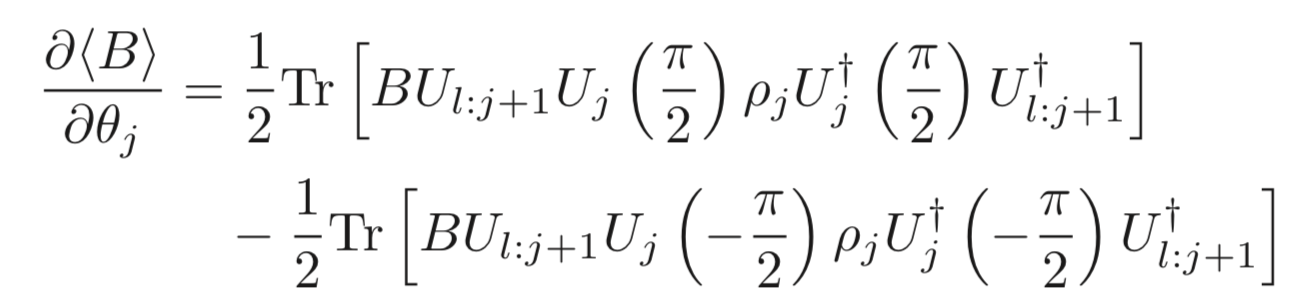
\includegraphics[width=\textwidth]{gradient.png}
  \end{frame}
  
  \begin{frame}
  	\frametitle{SVM}
  	\framesubtitle{Kernels}
  	\begin{itemize}
  	\item Linear classifier (e.g. perceptron): perform binary classification by separating labels in feature space with hyperplane.
  	\item Data is not always separable
  	\item Idea: Map data to higher dimensional space where data is separable
  	\item Kernel function does this implicitly by providing a means to compute the inner product in that space
  	\end{itemize}
  \end{frame}
  
  \begin{frame}
  	\frametitle{SVM}
  	\framesubtitle{Kernels}
  	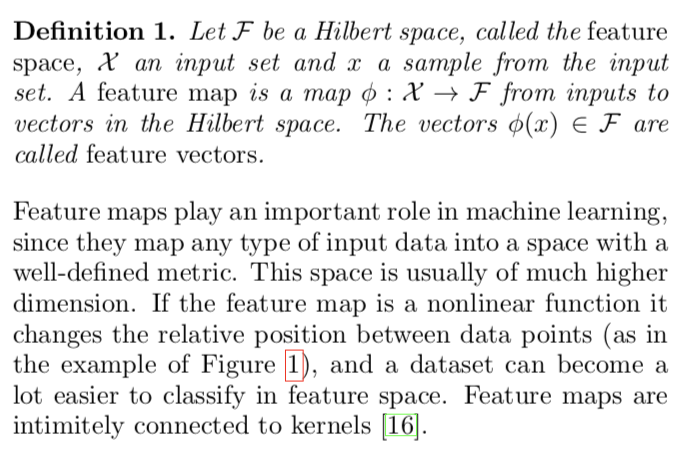
\includegraphics[width=\textwidth]{kernel_dfn_1.png}
  \end{frame}
  
  \begin{frame}
  	\frametitle{SVM}
  	\framesubtitle{Kernels}
  	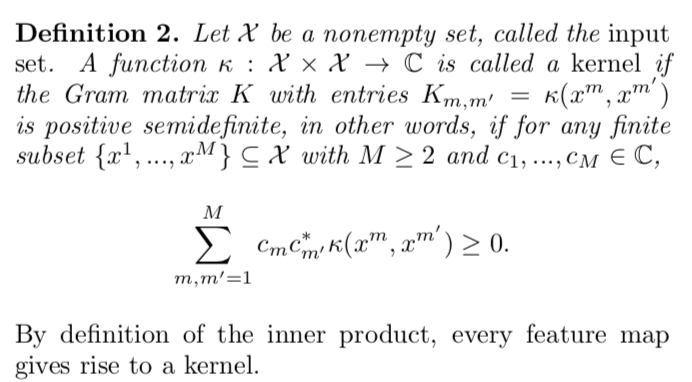
\includegraphics[width=\textwidth]{kernel_dfn_2.png}
  \end{frame}
  
  \begin{frame}
  	\frametitle{SVM}
  	\framesubtitle{Kernels}
  	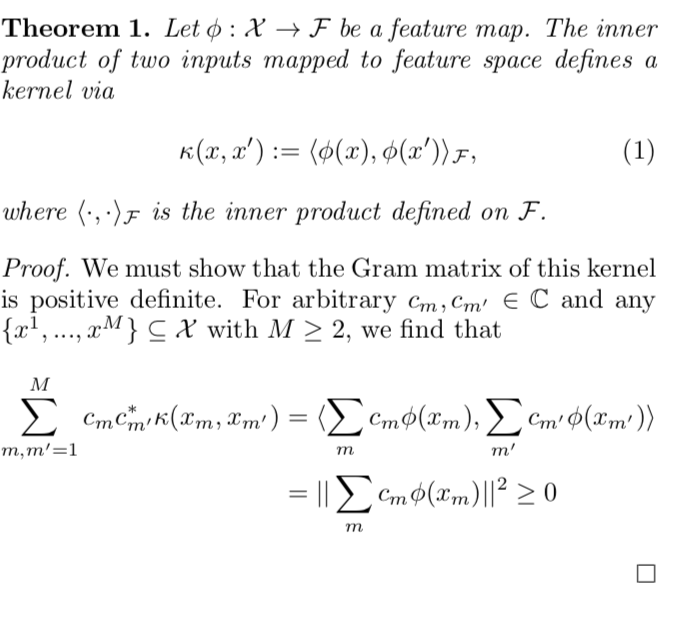
\includegraphics[width=0.8\textwidth]{kernel_dfn_3.png}
  \end{frame}
  
  \begin{frame}
  	\frametitle{SVM}
  	\framesubtitle{Kernels}
  	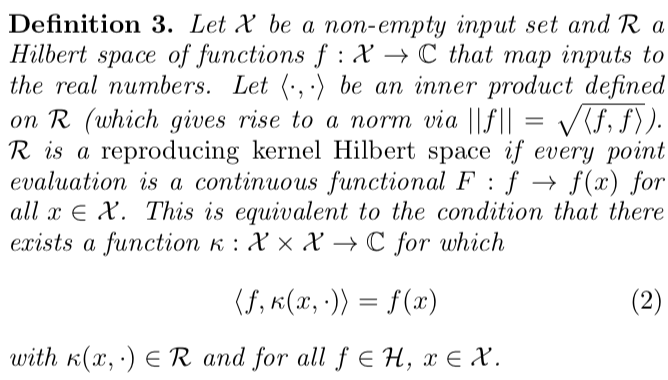
\includegraphics[width=0.8\textwidth]{kernel_dfn_4.png}
  \end{frame}
	\frametitle{SVM}
  	\framesubtitle{Kernels}
	\begin{frame}
	\begin{itemize}
	\item Can construct unique RKHS for any feature map
	\item Mercer's Theorem: If kernel $k$ is positive, we can expand $k$ (as a uniformly convergent series) in terms of eigenfunctions and eigenvalues of a positive operator that come from $k$.	
	\item Representer Theorem: Even if we’re trying to solve an optimization problem in an infinite dimensional space $H_k$ containing linear combinations of kernels centered on arbitrary $x_i$'s, then the solution lies in the span of the $n$ kernels centered on the $x_i$’s.
	\end{itemize}
	
	\end{frame}

	\begin{frame}
	\frametitle{SVM}
  	\framesubtitle{Optimization -- Dual Formulation}
  	
  	${\displaystyle {\begin{aligned}{\text{maximize}}\,\,f(c_{1}\ldots c_{n})&=\sum _{i=1}^{n}c_{i}-{\frac {1}{2}}\sum _{i=1}^{n}\sum _{j=1}^{n}y_{i}c_{i}(\varphi ({\vec {x}}_{i})\cdot \varphi ({\vec {x}}_{j}))y_{j}c_{j}\\&=\sum _{i=1}^{n}c_{i}-{\frac {1}{2}}\sum _{i=1}^{n}\sum _{j=1}^{n}y_{i}c_{i}k({\vec {x}}_{i},{\vec {x}}_{j})y_{j}c_{j}\\\end{aligned}}}$

	${\displaystyle {\text{subject to }}\sum _{i=1}^{n}c_{i}y_{i}=0,\,{\text{and }}0\leq c_{i}\leq {\frac {1}{2n\lambda }}\;{\text{for all }}i.}$
	
	\begin{itemize}
	\item Use quadratic programming, coordinate descent, gradient descent, SMO...
	\item Representer's Theorem
	\item Only ever need to evaluate inner product in RKHS to train and 	test model
	\end{itemize}

  	\end{frame}
  	
	\begin{frame}
	\frametitle{SVM}
  	\framesubtitle{Explicit Classification}
	\begin{itemize}
	\item Encode data, just as with QCL. This time, encode data under feature map transformation directly.
	\item $U_\phi(x) \ket{0}^N = \ket{\Phi(x)}$
	\item Hence, $K(x, z) = |\bra{\phi(x)}\ket{\phi(z)}|^2$
	\item Map must be hard to compute classically. Simple kernel like RBF allows efficient classical computation in infinite-dimensional Hilbert space. Large quantum Hilbert space is not enough.
	\end{itemize}
	
	\end{frame}
	
	\begin{frame}
	\frametitle{SVM}
  	\framesubtitle{Havlicek et al}
	\begin{itemize}
	\item Consider feature map $U_{\phi}(x) = V_{\phi(x)}H^{\otimes n}V_{\phi(x)}H^{\otimes n}$ where $V_{\phi(x)} = exp\Big(i \sum\limits_{S\subseteq [n]} \phi_S(x) \prod_{i \in S} Z_i\Big)$,  $|S| \leq 2$
	\item Conjecture: Classical evaluation of inner products generated from circuits with two basis changes and diagonal gates up to additive error is "hard"
	\pause
	\item $n = d = 2$ qubits
	\item $\phi_{\{i\}}(\vec{x}) = x_i$ and $\phi_{\{1,2\}} = (\pi - x_1)(\pi - x_2)$ with $\vec{x} \in (0, 2\pi]^2$
	\item Take some random unitary $V \in SU(4)$ and defined data "gap" $\Delta = 0.3$. 
	\item Then, we define $\bra{\Phi(x)} V^\dag Z_1 Z_2 V \ket{\Phi(x)} \geq \Delta \implies +1$ label and $-1$ otherwise
	\end{itemize}
	\end{frame}
	
	\begin{frame}
	\frametitle{SVM}
  	\framesubtitle{Havlicek et al}
	\begin{itemize}
	\item Now, apply $\theta$-parameterized layers of $l$ unitaries. $\theta \in \RR^{2N(l+1)}$
	\item For binary classication, $y \in \{ +1 , -1 \}$. 
	\item In our case, $\vec{f} = Z_1 Z_2$ and $0 \leq l \leq 4$
	\item Measure $ M_y = \frac{1}{2} (I + y \vec{f})$ with $\vec{f} = \sum_{z \in \{0, 1\}^N}f(z) \ket{z}\bra{z}$ and $f : \{ 0, 1\}^n \rightarrow \{ +1, -1 \}$
	\item Obtain empricial distribution $p_y(x)$ which is expectation of $M_y$ sampled with repeated shots
	\item Classify by comparing $p_y(+1)$ to $p_{-1}(x)$ (can add bias as well)
	\item Define loss function to be average number of missclassifications
	\end{itemize}
	\end{frame}
	
	\begin{frame}
	\frametitle{SVM}
  	\framesubtitle{Havlicek et al}
  	\begin{itemize}
  	\item How is this SVM?
  	\item Decision rule for label: $m(x) = sgn (\bra{\Phi(x)} W^\dag(\theta) \vec{f} W(\theta) \ket{\Phi(x)}$
  	\item Decompose density operator $\rho_{in}$ and $\rho_{out}$ in $Pauli$ product basis $\{P_\alpha\}$. 
  	\item Expectation value of binary measurement and decision rule can be expressed in terms of $w_\alpha(\theta) = \tr [W^\dag(\theta) \vec{f} W(\theta) P_\alpha]$ and $\Phi_\alpha(x) = \bra{\Phi(x)} P_\alpha\ket{\Phi(x)}$
  	\item $m(x) = sgn(1/2^N \sum_\alpha w_\alpha(\theta) \Phi_\alpha(x))$. SVM separating hyperplane.
  	\item Decomposition shows we should think of $\ket{\phi(x)}\bra{\phi(x)}$ as the feature vectors i.e. feature vectors don't live directly in the Hilbert space $H = (\CC^2)^{\otimes N}$. As expected, since global phase would make this problematic.
  	\end{itemize}
  	\end{frame}

\end{document}
